\documentclass{article}
\usepackage[margin=1.25in]{geometry}
\usepackage{amsmath, amssymb, setspace, enumerate, enumitem}
\usepackage{graphicx}
\usepackage[makeroom]{cancel}
\onehalfspacing

\begin{document}
    \begin{itemize}
        \item \textbf{Problem 7.9.} $G^0 = 0$. $G_1 = 1$ and $G_n = 7G_{n-1} - 12 G_{n-2}$ for $n > 1$. Compute $G_5$. Show $G_n = 4^n - 3^n$ for $n \geq 0$.\\
        \begin{tabular}{ |c|c|c|c|c|c|c| } 
            \hline
            $n$ & 0 & 1 & 2 & 3 & 4 & 5\\ 
            \hline
            $A_n$ & 0 & 1 & 7 & 37 & 175 & 781 \\
            \hline
        \end{tabular}
        \begin{enumerate}[label=(\roman*)]
            \item Prove the base case:
            \begin{align*}
                G(0) = 4^0 - 3^0 = 0
            \end{align*}
            \begin{center}
                base case is true\\
            \end{center}
            \item With induction hypothesis: assume $G(n) = 4^n - 3^n$, prove by direct proof that\\ $G(n) = 4^n - 3^n \rightarrow G(n+1) = 4^{n+1} - 3^{n+1}$ for all $n \geq 0$.
            \begin{align*}
                G(n + 1) &= 7G(n+1-1) - 12G(n+1-2) \text{ (recursive definition)}\\ 
                &= 7G(n) - 12G(n-1)\\
                7G(n) - 12G(n-1) &= 4^{n+1} - 3^{n+1}
            \end{align*}
            \begin{center}
                manipulate the LHS
            \end{center}
            \begin{align*}
                7G(n) - 12G(n-1) &= 7(4^{n} - 3^{n})  - 12(4^{n-1} - 3^{n-1})\text{ (induction hypothesis)}\\
                &= 7(4^n - 3^n) - \cancel{12}(\frac{4^n(3) - 3^n(4)}{\cancel{12}})\\
                &= 7(4^n - 3^n) - (3(4^n) - 4(3^n))\\
                &= 7(4^n) - 7(3^n) - 3(4^n) - 4(3^n)\\
                &= 4(4^n) - 3(3^n)\\
                &= 4^{n+1} - 3^{n+1}
            \end{align*}
            \begin{center}
                We prove the statement is true for $n \geq 0$ by direct proof $\hfill\blacksquare$
            \end{center}

        \end{enumerate}
        \item \textbf{Problem 7.12(c). (See Problem 7.28 for hints.)} Tinker to guess a formula for each recurrence and prove it. In each case $A_1 = 1$ and for $n > 1$:
        \begin{enumerate}[label=(c)]
            \item $A_n = 10nA_{n-1} / (n-1) + n$
            \newline
            \begin{tabular}{ |c|c|c|c|c| } 
                \hline
                $n$ & 2 & 3 & 4 & 5\\ 
                \hline
                $A_n$ & 22 & 333 & 4444 & 55555 \\
                \hline
            \end{tabular}
            \begin{enumerate}[label=\roman*.]
                \item formula found:
                \begin{align*}
                    \frac{10^n-1}{9}n
                \end{align*}
                \item prove the base case:
                \begin{align*}
                    A(2) &= \frac{100-1}{9}(2)\\
                         &= \frac{99}{9}(2) = 22
                \end{align*}
                \begin{center}
                    base case proven
                \end{center}
                \item With induction hypothesis: assume $A(n) = \frac{10^n - 1}{9}n$, prove by direct proof that $A(n) = \frac{10^n - 1}{9}n \rightarrow A(n+1) = \frac{10^{n+1} - 1}{9}(n+1)$ for all $n > 0$.
                \begin{align*}
                    A(n) &= \frac{10nA(n-1)}{n-1}+n\\
                    A(n+1) &= \frac{10(n+1)A(n)}{n} + (n+1) \text{ (recursive definition)}
                \end{align*}
                \begin{center}
                    with with RHS
                \end{center}
                \begin{align*}
                    A(n+1) &= \frac{10(n+1)A(n)}{n} + (n+1) \text{ (induction hypothesis)}\\
                    &= \frac{10(n+1)(\frac{10^n-1}{9}\cancel{n})}{\cancel{n}} + (n+1)\\
                    &= \frac{10(n+1)(10^n-1)}{9} + (n+1)\\
                    &= \frac{(10n+10)(10^n-1) + 9(n+1)}{9}\\
                    &= \frac{10n(10^n) - 10n + 10(10^n) - 10 + 9n + 9}{9}\\
                    &= \frac{10n(10^n) - n + 10^{n+1} - 1}{9}\\
                    &= \frac{10^{n+1}n - n + 10^{n+1} - 1}{9}\\
                    &= \frac{10^{n+1} - 1}{9}(n+1)
                \end{align*}
                \item we prove by direct proof that the statement is true for all $n > 1$ $\hfill \blacksquare$
            \end{enumerate}
        \end{enumerate}
        \item \textbf{Problem 7.13(a).} Analyze these very fast growing recursions. [Hint: Take logarithms.]
        \begin{enumerate}[label=(a)]
            \item $M_1 = 2$ and $M_n = aM^2_{n-1}$ for $n>1$. Guess and prove a formula for $M_n$. Tinker, tinker.
            \begin{tabular}{ |c|c|c|c|c| } 
                \hline
                $n$ & 2 & 3 & 4 & 5\\ 
                \hline
                $A_n$ & a4 & a16 & a256 & a65536 \\
                \hline
            \end{tabular}
            \begin{enumerate}[label=(\roman*)]
                \item formula found:
                \begin{align*}
                    M(n) = 2^{2^{n-1}}\\
                \end{align*}
                \item base case:
                \begin{align*}
                    M(2) &= a(2^{2^1})\\
                         &= a(2^2)\\
                         &= a4
                \end{align*}
                \begin{center}
                    base case proven
                \end{center}
                \item prove using direct proof
                \begin{align*}
                    aM(n-1)^2 &= a2^{2^{n-1}}\\
                    M(n-1)^2 &= 2^{2^{n-1}} \text{ simplify}\\
                    \log_{2}(M(n-1)^2) &= \log_2(2^{2^{n-1}}) \text{ log both sides}\\
                    \log_{2}(M(n-1)^2) &= 2^{2^{n-1}}
                \end{align*}
                \begin{center}
                    work with LHS
                \end{center}
                \begin{align*}
                    \log_{2}(M(n-1)^2) & = 2 \log_{2}(M(n-1))\\
                                       & = 2 \log_{2}(2^{2^{(n-1) - 1}})\\
                                       & = 2(2^{n-2})\\
                                       & = 2^{n-1}
                \end{align*}
                \item we prove by direct proof that the statement is true for all $n > 0$ $\hfill\blacksquare$
            \end{enumerate}
        \end{enumerate}
        \item \textbf{Problem 7.19(d).} Recall the Fibonacci numbers: $F_1$, $F_2 = 1$; and, $F_n = F_{n-1} + F_{n-2}$ for $n > 2$
        \begin{enumerate}[label=(d)]
            \item Prove that every third Fibonacci number, $F_{3n}$, is even
            \begin{enumerate}[label=(\roman*)]
                \item We have to prove that $F_{3n} = 2p$, for some $p \in \mathbb{N}$
                \item prove the base case:
                \begin{align*}
                    F_{3n-1} &= F_2 \text{ when $n=1$, } \rightarrow F_2 = 1\\
                    F_{3n-2} &= F_1 \text{ when $n=1$, } \rightarrow F_1 = 1
                \end{align*}
                \item since the fibonacci sequence is a sum of the previous two terms, we can make the following assumptions:
                \begin{center}
                    By the given formula $F_n = F_{n-1} + F_{n-2}$, we can calculate $F_{3n} = F_{3n-1} + F_{3n-2}$\\
                    We know that both $F_{3n-1}$ and $F_{3n-2}$ are sums of even and odd numbers
                \end{center}
                \begin{align*}
                    F_{3n-1} &= 2k + (2j + 1)\\
                             &= 2(k + j) + 1\\
                    F_{3n-2} &= (2w + 1) + 2i\\
                             &= 2(w + i) + 1
                \end{align*}
                \begin{center}
                    plugging back into the original function, we get:
                \end{center}
                \begin{align*}
                    F_{3n} &= [2(k+j) + 1] + [2(w+i) + 1]\\
                           &= 2(k + j) + 2(w+i) + 2\\
                           &= 2(k + j + w + i + 1)
                \end{align*}
                \begin{center}
                    We prove that the statement is true for all $n > 2$ $\hfill\blacksquare$
                \end{center}
            \end{enumerate}
        \end{enumerate}
        \item \textbf{Problem 7.42.} Give pseudocode for a recursive function that computes $3^{2^n}$ on input $n$.
        \begin{center}
            Code example:
        \end{center}
        \begin{verbatim}
            int f(int n):
                if n is 0 return 3
                else return f(n-1) squared
        \end{verbatim}
        \begin{center}
            Mathematical function:
        \end{center}
        \begin{align*}
            T_0 &= 3\\
            T_n &= (T_{n-1})^2
        \end{align*}
        \begin{enumerate}[label=(\alph*)]
            \item Prove that your function correctly computes $3^{2^n}$ for every $n \geq 0$.\\
            \begin{tabular}{ c|c|c|c|c|c }
                $n$ & 0 & 1 & 2 & 3 & 4\\
                \hline
                $T_n$ & 3 & 9 & 81 & 6561 & 43046721\\
            \end{tabular}
            \begin{enumerate}[label=(\roman*)]
                \item prove the base case for $n = 1$
                \begin{align*}
                    T(n) &= T(n-1)^2\\
                    T(1) &= T(0)^2\\
                         &= 9
                \end{align*}
                \item prove using a direct proof
                \begin{center}
                    $T(n) = 3^{2^n}$\\$T(n) = T(n-1)^2$
                \end{center}
                \begin{align*}
                    T(n-1)^2 &= 3^{2^n}\\
                    (3^{2^{n-1}})^2 &= 3^{2^n} \text{ log both sides}\\
                    \log{3}((3^{2^{n-1}})^2) &= \log{3}(3^{2^n})\\
                    2\log{3}(3^{2^{n-1}}) &= \log{3}(3^{2^n})\\
                    2(2^{n-1}) &= 2^n\\
                    \text{LHS: } 2(2^{n-1}) &= 2^{n-1+1}\\
                    &= 2^n
                \end{align*}
                \item we prove by a direct proof that our function computes $3^{2^n}$ for every $n \geq 0$ $\hfill\blacksquare$
            \end{enumerate}
            \item Obtain a recurrence for the runtime $T_n$. Guess and prove a formula for $T_n$.
            \begin{enumerate}[label=(\roman*)]
                \item runtime $T_n$
                \begin{itemize}[label=$\bullet$]
                    \item assume squaring a number is passed onto a function such as:
                    \begin{verbatim}
                        int square(int n) {
                            return n * n;
                        }
                        // two steps in total 
                        // (1) multiplication 
                        // (2) return
                    \end{verbatim}
                    \item $T_0 = 2$, when $n$ is 0 $\rightarrow$ (test, return)
                    \item $T_1 = 6$, when $n$ is 1 $\rightarrow$ (test, multiplication(2), set, and $T_0$)
                    \item $T_2 = 10$, when $n$ is 2 $\rightarrow$ (test, multiplication(2), set, and $T_1$)
                    \item $T_n = T_{n-1} + 4$ for $n \geq 2$ 
                \end{itemize}
                \item derived formula: $T_n = 4n + 2$
                \begin{center}
                    base case: $n=1$
                \end{center}
                \begin{align*}
                    T(1) &= 4(1) + 2\\
                         &= 6
                \end{align*}
                \begin{center}
                    prove by direct proof
                \end{center}
                \begin{align*}
                    T(n) &= T(n-1) + 4\\
                    T(n) &= 4n + 2
                \end{align*}
                \begin{center}
                    Setting both equations equal, we get
                \end{center}
                \begin{align*}
                    T(n-1) + 4 &= 4n + 2\\
                    \text{LHS $\rightarrow$ } T(n-1) + 4 &= 4(n-1 + 2 + 4)\\
                    &= 4n \cancel{-4} + 2 \cancel{+4}\\
                    &= 4n + 2
                \end{align*}
                \item we prove by direct proof that our formula $T_n$ accurately calculates the runtime $T_n$ for $n \geq 1$ $\hfill\blacksquare$
            \end{enumerate}
        \end{enumerate}
        \item \textbf{Problem 7.45(c).} Give recursive definitions for the set $S$ in each of the following cases.
        \begin{enumerate}[label=(c)]
            \item $S =$ \{all strings with the same number of 0's and 1's\} (e.g. 0011,0101,100101).
            \begin{enumerate}[label=\arabic*.]
                \item \textbf{[basis]} $\epsilon \in S, 0 \in S, 1 \in S$
                \item \textbf{[constructor(i)]} $\epsilon \in S \rightarrow 0 \bullet x \bullet 0 \in S$;\\
                \textbf{[constructor(ii)]} $\epsilon \in S \rightarrow 1 \bullet x \bullet 1 \in S$.
            \end{enumerate}
        \end{enumerate}
        \item \textbf{Problem 7.49.} There are 5 rooted binary trees (RBT) with 3 nodes. How many have 4 nodes\\
        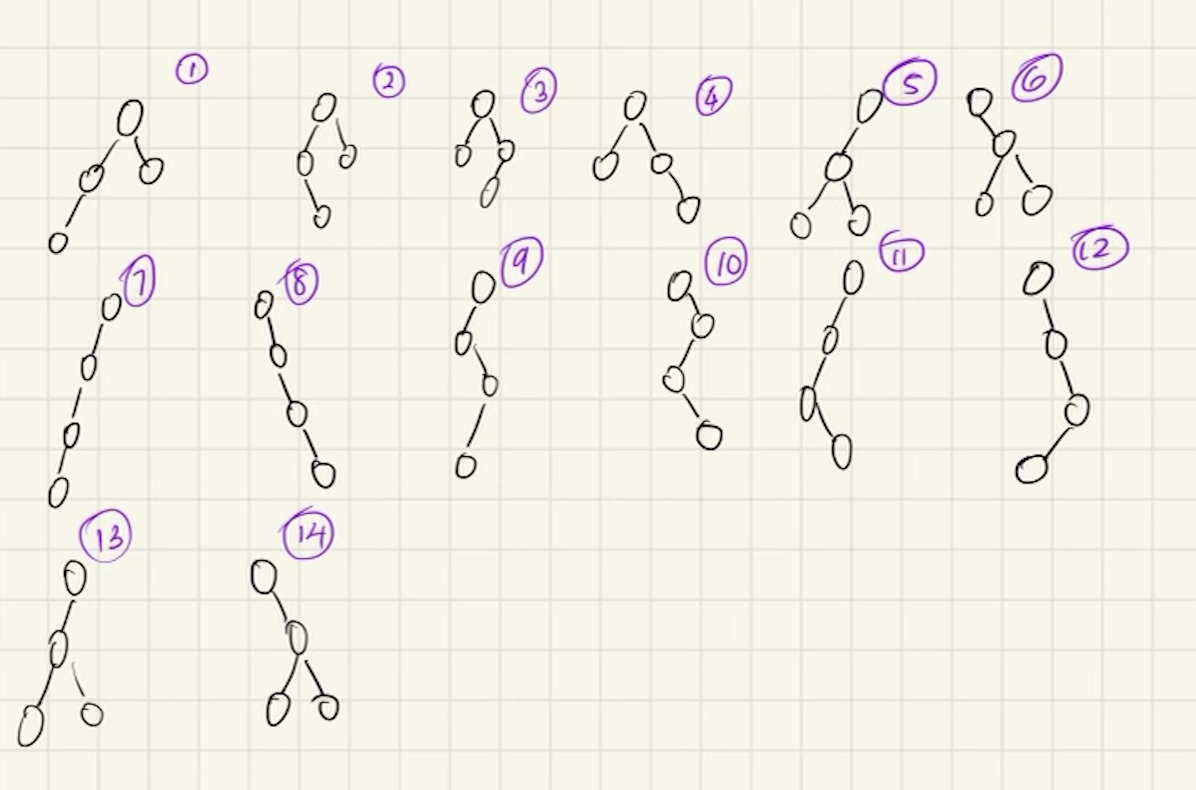
\includegraphics[width=100mm,scale=0.5]{binaryTrees.png}
        \begin{itemize}[label=$\bullet$]
            \item We can make 14 possible rooted binary trees with 4 nodes.
        \end{itemize}
        \item \textbf{Problem 8.12(d).} A set $P$ of parenthesis strings have a recursive definition.
        \begin{enumerate}[label=\arabic*.]
            \item $\epsilon \in P$
            \item $x \in P \rightarrow [x] \in P$\\
            $x,y \in P \rightarrow xy \in P$
        \end{enumerate}
        \begin{enumerate}[label=(d)]
            \item Prove by structural induction that every string $P$ is balanced.
            \begin{enumerate}[label=\roman*.]
                \item \textbf{[Base case]} When $n=1$ and $s_1 = \epsilon$, it is clearly balanced, $P(1)$ is true
                \item \textbf{[Induction step]} We prove that each constructor preserves palindromicity.\\
                If $x$ is a palindrome, that means $x^R$ will be in $P$, or $x^R =x$. This is our induction hypothesis.
                \begin{enumerate}[label=\arabic*.]
                    \item For constructor (i), we must show that $([x])^R = ([x])$.\\
                    We can rewrite $[x]$ as $[\bullet x \bullet]$\\
                    $([x])^R = [^R \bullet x^R \bullet ]^R = [\bullet x^R \bullet ] = [\bullet x \bullet] = [x]$\\
                    A potential set of this could be:\\
                    $P = {\epsilon, [], [[]], [[[]]], ...}$, all preserving palindromicity.
                    \item For constructor(ii), we must show that $(xy)^R = xy$.\\
                    We can rewrite $xy$ as $x \bullet y$\\
                    $(x \bullet y)^R = x^R \bullet y^R = x \bullet y = xy$\\
                    A potential set of this could be:
                    $P = {\epsilon, [], [][], [][][][], ...}$, all preserving palindromicity.
                \end{enumerate}
                \item By structural induction, we prove that every string $P$ is balanced given the constructors $\hfill\blacksquare$.
            \end{enumerate}
        \end{enumerate}
        \item \textbf{Problem 8.14.} A set $A$ is defined recursively as shown.
        \begin{enumerate}[label=\arabic*.]
            \item $3 \in A$.
            \item $x,y \in A \rightarrow x + y \in A$;\\
            $x,y \in A \rightarrow x-y \in A$.
        \end{enumerate}
        \begin{enumerate}[label=(\alph*)]
            \item Prove that every element of $A$ is a multiple of 3.
            \begin{enumerate}[label=\arabic*.]
                \item Prove by structural induction that every element in $A$ is a multiple of $3$.
                \item \textbf{[Base case]} for P(0), we have both:
                \begin{align*}
                    3 + 3 \in A &= 6\\
                    3 - 3 \in A &= 0
                \end{align*}
                \begin{center}
                    both are multiples of 3
                \end{center}
                \item \textbf{[Induction step]} suppose $x, y \in A$ and both $x$ and $y$ are multiples of 3
                \begin{align*}
                    x &= 3k\\
                    y &= 3k
                \end{align*}
                \begin{center}
                    the constructor rules allow us to create the following formula:
                \end{center}
                \begin{align*}
                    x + y &\in A\\
                    3k + 3w &\in A\\
                    3(k+w) &\in A
                \end{align*}
                \begin{center}
                    Adding two numbers that are multiples of 3 will always result in a number that is a multiple of 3
                \end{center}
                \item By structural induction, we conclude that ever member of $A$ is a multiple of $3\hfill\blacksquare$
            \end{enumerate}
            \item Prove that every multiple of 3 is in $A$.
            \begin{enumerate}[label=\arabic*.]
                \item We prove by contradiction that every multiple of 3 is in $A$. Consider m, a multiple of 3 that is not in $A$.
                \item \textbf{[Case 1]} $k > 0$, $m = 3k$, where $m$ is the largest multiple of 3 NOT in our set $A$.
                \begin{align*}
                    3k = 3 + 3 + 3 + ...
                \end{align*}
                \begin{center}
                    We can consider $3(k+1)$, which we know is in our set since it is larger than $m$
                \end{center}
                \begin{align*}
                    3(k+1) = 3k+3
                \end{align*}
                \begin{center}
                    We know by constructor(ii) that $x-y \in A$, and we know that $3 \in A$ by the basis.
                \end{center}
                \begin{align*}
                    3(k) &= x - y \text{, where } x = 3k + 3 \text{ and } y = 3\\
                         &= 3k + 3 - 3\\
                         &= 3k \text{ woops, we derived a contradiction!}
                \end{align*}
                \item \textbf{[Case 2]} $k < 0$, $m = -3k$, where $m$ is the smallest multiple of 3 NOT in our set A.
                \begin{align*}
                    3(-k) = -3 -3 -3 -3 -3 -3 -...
                \end{align*}
                \begin{center}
                    We can consider $3(-k - 1)$, which we know is in our set since it is smaller than $m$
                \end{center}
                \begin{align*}
                    3(-k-1) = -3k-3
                \end{align*}
                \begin{center}
                    We know by constructor(i) that $x+y \in A$, and we know that $3 \in A$ by the basis.
                \end{center}
                \begin{align*}
                    -3k &= x+y \text{, where } x = -3k -3 \text{ and } y = 3\\
                        &= -3k -3 + 3\\
                        &= -3k \text{ woops, we derived a contradiction!}
                \end{align*}
                \item \textbf{[Case 3]} $k = 0$, $m = 0$, $0$ is not in $A$
                \begin{center}
                    We know from the basis that $x = 3$ and $y = 3$\\
                    From constructor(ii), we can use $x - y$, where:
                \end{center}
                \begin{align*}
                    x - y &\in A\\
                    3 - 3 &\in A\\
                    0 &\in A \text{ woops, we derived a contradiction!}
                \end{align*}
                \item We prove by contradiction for 3 distinct cases of $k$, proving that all multiples of 3 is in $A \hfill\blacksquare$
            \end{enumerate}
        \end{enumerate}
    \end{itemize}
    
\end{document}